\documentclass[11pt,a4paper]{article}

% ── Packages ──────────────────────────────────────────────────────────────────
\usepackage[utf8]{inputenc}
\usepackage[a4paper,top=0.55in,bottom=0.55in,left=0.75in,right=0.75in]{geometry}
\usepackage{amsmath,amssymb}
\usepackage{booktabs}
\usepackage[ruled,vlined]{algorithm2e}
\usepackage{xcolor}
\usepackage{hyperref}
\usepackage{float}
\usepackage{caption}
\usepackage{parskip}
\usepackage{tikz}
\usepackage{pgfplots}
\pgfplotsset{compat=1.18}
\usetikzlibrary{shapes.geometric,arrows.meta,arrows,positioning,calc}

% ── Hyperref ──────────────────────────────────────────────────────────────────
\hypersetup{colorlinks=true,linkcolor=blue,urlcolor=cyan,citecolor=blue}

% ── Title ─────────────────────────────────────────────────────────────────────
\title{\textbf{Amenity Scoring System}\\[4pt]
       \large Feature Engineering \& Validation Report}
\author{}
\date{\today}

% ══════════════════════════════════════════════════════════════════════════════
\begin{document}
\maketitle

% ─────────────────────────────────────────────────────────────────────────────
\section{Executive Summary}
% ─────────────────────────────────────────────────────────────────────────────

This report describes an amenity scoring system that converts geographic coordinates into urban quality scores. The system queries 220+ Point-of-Interest (POI) types from OpenStreetMap, extracts 280 features across six dimensions, and outputs a 0--100 amenity index with a Metro / Urban / Rural classification.

\medskip
\noindent\textbf{Key capabilities:}
\begin{itemize}
  \item Validated on \textbf{1,010 locations} across India (Metro, Urban, Rural)
  \item Scores a location in 2--5 s (cached: $<$0.01 s)
  \item Robust retry logic handles OSM API rate limits and network instability
  \item 280 features covering density, proximity, quality, accessibility, spatial distribution, and economic balance
  \item Score breakdowns across 11 amenity categories
\end{itemize}

% ─────────────────────────────────────────────────────────────────────────────
\section{Introduction}
% ─────────────────────────────────────────────────────────────────────────────

\subsection{Problem Statement}

Simple urban quality assessments rely on subjective judgements or raw POI counts. These approaches miss several important factors:

\begin{itemize}
  \item \textbf{Accessibility:} 100 hospitals at 5 km is worse than 5 hospitals within 500 m.
  \item \textbf{Quality:} 10 basic clinics $\neq$ 1 multi-specialty hospital.
  \item \textbf{Spatial pattern:} Clustered amenities (walkable) vs.\ scattered amenities (car-dependent).
  \item \textbf{Balance:} Mono-use zones (only offices) vs.\ mixed-use areas (offices + retail + services).
\end{itemize}

\subsection{Solution Approach}

The system addresses these gaps through four components:

\begin{enumerate}
  \item \textbf{Feature engineering} --- 280 features covering density, proximity, quality, accessibility, spatial patterns, and economic balance.
  \item \textbf{Theory-based scoring} --- Weber-Fechner Law (density), Alonso's Bid-Rent Theory (proximity), Reilly's Law of Retail Gravitation (accessibility).
  \item \textbf{Spatial analysis} --- Nearest Neighbor Index (NNI) and Moran's~I to identify walkable clustering vs sprawl.
  \item \textbf{Penalty system} --- Additive penalties (capped at 50\%) for low data quality, unequal distribution, and low diversity.
\end{enumerate}

% Pipeline diagram
\begin{figure}[H]
\centering
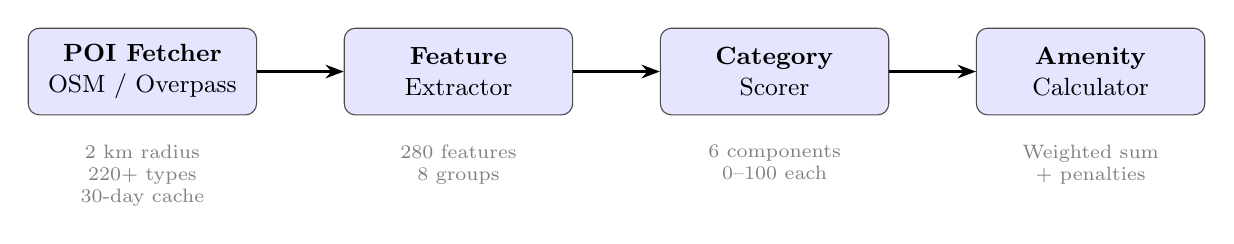
\begin{tikzpicture}[
  box/.style={rectangle, rounded corners=4pt, draw=black!70, fill=blue!10,
              minimum width=2.9cm, minimum height=1.1cm, align=center, font=\small},
  sub/.style={font=\scriptsize, text=gray, align=center},
  arr/.style={-{Stealth}, thick}
]
  \node[box] (A) {\textbf{POI Fetcher}\\OSM / Overpass};
  \node[box, right=1.1cm of A] (B) {\textbf{Feature}\\Extractor};
  \node[box, right=1.1cm of B] (C) {\textbf{Category}\\Scorer};
  \node[box, right=1.1cm of C] (D) {\textbf{Amenity}\\Calculator};

  \draw[arr] (A)--(B); \draw[arr] (B)--(C); \draw[arr] (C)--(D);

  \node[sub, below=0.25cm of A] {2 km radius\\220+ types\\30-day cache};
  \node[sub, below=0.25cm of B] {280 features\\8 groups};
  \node[sub, below=0.25cm of C] {6 components\\0--100 each};
  \node[sub, below=0.25cm of D] {Weighted sum\\+ penalties};
\end{tikzpicture}
\caption{End-to-end processing pipeline}
\end{figure}

% ─────────────────────────────────────────────────────────────────────────────
\section{Data Collection}
% ─────────────────────────────────────────────────────────────────────────────

\subsection{Data Source}

\begin{tabular}{@{}ll@{}}
  \textbf{Source}   & OpenStreetMap via Overpass API (open-source, global, no cost) \\
  \textbf{Radius}   & 2{,}000 m --- captures walkable, bikeable, and short-drive amenities \\
  \textbf{Query}    & Single comprehensive request for all 220+ POI types \\
  \textbf{Resilience} & Smart retry logic (up to 10 attempts) handles API rate limits \\
  \textbf{Cache}    & 30-day local cache; 95\%+ hit rate (2--5 s $\to$ $<$0.01 s per location)
\end{tabular}

\subsection{Amenity Categories}

POIs are grouped into 11 categories based on Maslow's Hierarchy of Needs --- basic needs weighted highest, lifestyle needs weighted lowest.

\begin{table}[H]
\centering
\caption{Amenity categories, coverage, and scoring weights}
\begin{tabular}{@{}llr@{}}
\toprule
\textbf{Category} & \textbf{Representative POI types} & \textbf{Weight} \\ \midrule
Essential   & Grocery, pharmacy, police, fuel (14 types)          & 24\% \\
Healthcare  & Hospital, clinic, doctors, dentist (13 types)       & 17\% \\
Education   & University, school, coaching, library (11 types)    & 14\% \\
Transport   & Metro, bus stop, taxi, parking (17 types)           & 11\% \\
Finance     & Bank, ATM, post office, insurance (9 types)         & 9\%  \\
Shopping    & Mall, supermarket, retail shops (60+ types)         & 8\%  \\
Food        & Restaurant, caf\'{e}, fast food (25 types)          & 5\%  \\
Cultural    & Museum, park, theatre, temple (23 types)            & 4\%  \\
Premium     & Hotel, gym, spa, golf course (18 types)             & 3\%  \\
Employment  & Office, coworking, factory, IT park (16 types)      & 3\%  \\
Civic       & Town hall, courthouse, embassy (14 types)           & 2\%  \\ \midrule
\textbf{Total} & \textbf{220+ POI types} & \textbf{100\%} \\ \bottomrule
\end{tabular}
\end{table}

% Category weight bar chart
\begin{figure}[H]
\centering
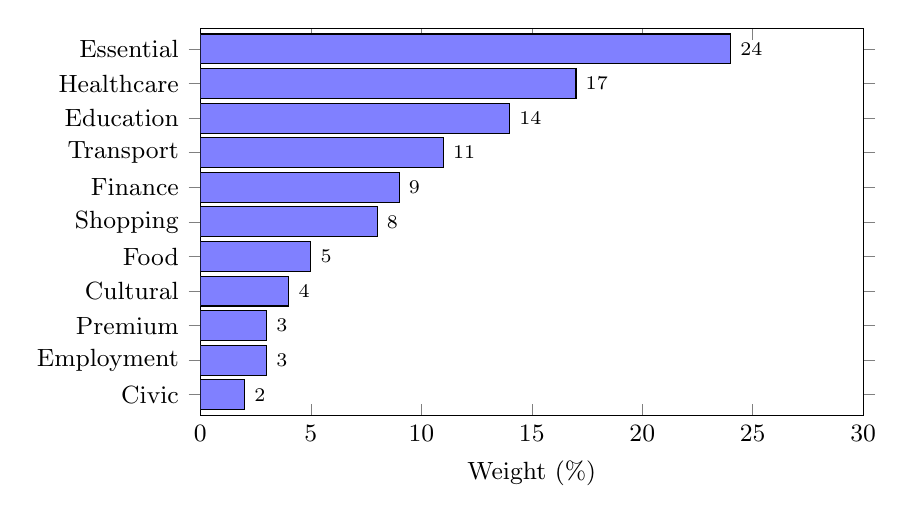
\begin{tikzpicture}
\begin{axis}[
  xbar, width=10cm, height=6.5cm, bar width=0.38cm,
  xlabel={Weight (\%)},
  symbolic y coords={Civic,Employment,Premium,Cultural,Food,Shopping,Finance,Transport,Education,Healthcare,Essential},
  ytick=data, xmin=0, xmax=30,
  nodes near coords, nodes near coords align={horizontal},
  every node near coord/.style={font=\scriptsize},
  tick label style={font=\small}, label style={font=\small},
  enlarge y limits=0.06,
]
\addplot[fill=blue!50] coordinates {
  (2,Civic)(3,Employment)(3,Premium)(4,Cultural)(5,Food)
  (8,Shopping)(9,Finance)(11,Transport)(14,Education)(17,Healthcare)(24,Essential)
};
\end{axis}
\end{tikzpicture}
\caption{Category weights (Maslow-based priority, highest = most essential)}
\end{figure}

% ─────────────────────────────────────────────────────────────────────────────
\section{Feature Engineering}
% ─────────────────────────────────────────────────────────────────────────────

\subsection{Feature Taxonomy}

The 280 features used in scoring are organised into eight groups:

\begin{center}
\begin{tabular}{@{}lrl@{}}
\toprule
\textbf{Group} & \textbf{Count} & \textbf{Purpose} \\ \midrule
Density          & 110 & POI counts and densities at 500 m, 1 km, 2 km \\
Proximity        & 55  & Nearest and average distances per category \\
Quality          & 33  & Premium-to-basic ratios per category \\
Accessibility    & 11  & Gravity-model score per category \\
Spatial          & 24  & NNI, Moran's~I, DBSCAN, hotspot intensity \\
Economic         & 11  & POI-mix alignment with target distribution \\
Global metrics   & 2   & Simpson diversity, Gini coefficient \\
Density gradients& 33  & Cross-radius sprawl detection \\ \midrule
\textbf{Total}   & \textbf{280} & \\ \bottomrule
\end{tabular}
\end{center}

\subsection{Core Per-Category Features}

\subsubsection{Density (Multi-Radius)}

At each radius $r \in \{500\,\text{m},\,1{,}000\,\text{m},\,2{,}000\,\text{m}\}$:

\begin{align}
\text{Count}_r   &= \bigl|\{p : d(\text{loc},\,p) \le r\}\bigr| \\[4pt]
\text{Density}_r &= \frac{\text{Count}_r}{\pi r^2} \quad [\text{POIs km}^{-2}]
\end{align}

Using multiple radii reveals the urban structure: high density at all radii indicates a city core; density that drops beyond 500 m indicates an isolated area; low density near the centre but high density further out indicates sprawl.

% Density gradient pattern diagram
\begin{figure}[H]
\centering
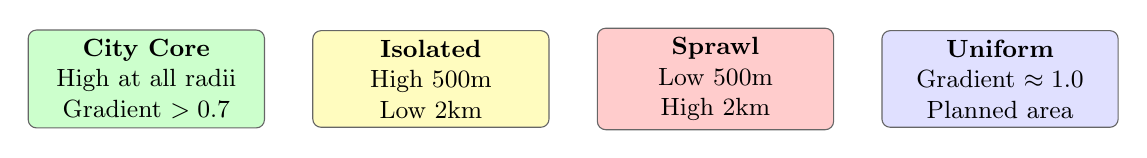
\begin{tikzpicture}[
  pat/.style={rectangle, rounded corners=3pt, draw=black!60,
              minimum width=3.0cm, minimum height=1.0cm, align=center, font=\small}
]
  \node[pat, fill=green!20]  (A) {\textbf{City Core}\\High at all radii\\Gradient $>0.7$};
  \node[pat, fill=yellow!25, right=0.6cm of A] (B) {\textbf{Isolated}\\High 500m\\Low 2km};
  \node[pat, fill=red!20,    right=0.6cm of B] (C) {\textbf{Sprawl}\\Low 500m\\High 2km};
  \node[pat, fill=blue!12,   right=0.6cm of C] (D) {\textbf{Uniform}\\Gradient $\approx1.0$\\Planned area};
\end{tikzpicture}
\caption{Density gradient patterns detected by cross-radius analysis}
\end{figure}

\subsubsection{Proximity}

Distances are computed with the Haversine formula:

\begin{equation}
d = 2R\arcsin\!\left(\sqrt{\sin^2\!\tfrac{\Delta\phi}{2}
    + \cos\phi_1\cos\phi_2\sin^2\!\tfrac{\Delta\lambda}{2}}\right),
    \quad R = 6{,}371\,\text{km}
\end{equation}

\begin{align}
d_{\min}  &= \min_{i}\; d(\text{loc},\,p_i) \\
d_{\text{avg}} &= \frac{1}{n}\sum_{i=1}^{n} d(\text{loc},\,p_i)
\end{align}

Nearest distance reflects how quickly a POI can be reached; average distance reflects general convenience.

\subsubsection{Quality Ratio}

\begin{equation}
r_{\text{qual}} = \frac{N_{\text{premium}}}{N_{\text{basic}} + 1}
\end{equation}

Examples: Healthcare $= \text{hospitals}/(\text{clinics}+1)$; Education $= \text{universities}/(\text{schools}+1)$; Shopping $= \text{malls}/(\text{kirana stores}+1)$.

Higher-tier amenities indicate better service quality; the $+1$ in the denominator prevents division by zero.

\subsection{Advanced Spatial Features}

\subsubsection{Nearest Neighbor Index (NNI)}

NNI measures whether POIs are more clustered or spread out than a random distribution:

\begin{equation}
\text{NNI} = \frac{\bar{d}_{\text{obs}}}{\bar{d}_{\text{exp}}}
\end{equation}

\begin{align}
\bar{d}_{\text{obs}} &= \frac{1}{n}\sum_{i=1}^{n}\min_{j\neq i} d(p_i,p_j) \\[4pt]
\bar{d}_{\text{exp}} &= \frac{0.5}{\sqrt{n/A}}, \quad A = \pi\times 2^2 = 12.57\,\text{km}^2
\end{align}

\begin{center}
\begin{tabular}{@{}ll@{}}
\toprule
\textbf{NNI range} & \textbf{Interpretation} \\ \midrule
$< 0.5$      & Highly clustered --- may indicate car-dependent development \\
$0.5 - 1.0$  & Moderate clustering --- good for walkable areas \\
$\approx 1.0$& Random distribution --- typical of low-density suburbs \\
$> 1.5$      & Spread out --- sprawl \\ \bottomrule
\end{tabular}
\end{center}

% NNI scoring curve
\begin{figure}[H]
\centering
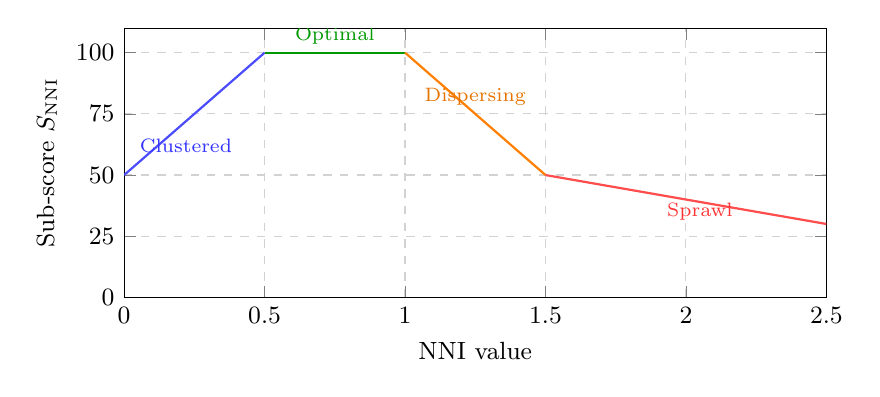
\begin{tikzpicture}
\begin{axis}[
  width=10.5cm, height=5cm,
  xlabel={NNI value}, ylabel={Sub-score $S_{\text{NNI}}$},
  xmin=0, xmax=2.5, ymin=0, ymax=110,
  xtick={0,0.5,1.0,1.5,2.0,2.5}, ytick={0,25,50,75,100},
  grid=major, grid style={dashed,gray!35},
  tick label style={font=\small}, label style={font=\small},
]
\addplot[blue!70,  thick, domain=0:0.5,   samples=40] {50+(x/0.5)*50};
\addplot[green!60!black, thick, domain=0.5:1.0,  samples=10] {100};
\addplot[orange,   thick, domain=1.0:1.5,  samples=40] {100-((x-1.0)/0.5)*50};
\addplot[red!70,   thick, domain=1.5:2.5,  samples=40] {max(0,50-(x-1.5)*20)};
\node[font=\scriptsize,blue!80]         at (axis cs:0.22,62)  {Clustered};
\node[font=\scriptsize,green!60!black]  at (axis cs:0.75,107) {Optimal};
\node[font=\scriptsize,orange!90!black] at (axis cs:1.25,82)  {Dispersing};
\node[font=\scriptsize,red!80]          at (axis cs:2.05,35)  {Sprawl};
\end{axis}
\end{tikzpicture}
\caption{NNI sub-score: optimal range 0.5--1.0 scores 100; scores drop for over-clustering or sprawl}
\end{figure}

\subsubsection{Moran's I (Spatial Autocorrelation)}

Moran's~I measures whether nearby POIs tend to be similar to each other:

\begin{equation}
I = \frac{n}{{\displaystyle\sum_i\sum_j w_{ij}}}
    \cdot
    \frac{{\displaystyle\sum_i\sum_j w_{ij}(x_i-\bar{x})(x_j-\bar{x})}}
         {{\displaystyle\sum_i(x_i-\bar{x})^2}}
\end{equation}

Spatial weights use inverse distance, normalised per row:

\begin{equation}
w_{ij} = \frac{1/d_{ij}}{\displaystyle\sum_k 1/d_{ik}}
\end{equation}

\begin{center}
\begin{tabular}{@{}ll@{}}
\toprule
\textbf{Value} & \textbf{Interpretation} \\ \midrule
$I \approx +1$ & Similar POIs cluster together --- single-use zones \\
$I \approx 0$  & Random pattern --- mixed-use areas \\
$I \approx -1$ & Similar POIs are spread apart --- even distribution \\ \bottomrule
\end{tabular}
\end{center}

\subsubsection{DBSCAN Clustering}

DBSCAN finds natural POI clusters without needing to specify the number of clusters in advance.

\begin{algorithm}[H]
\caption{DBSCAN --- POI hub detection}
\KwIn{POI coordinates; $\varepsilon = 0.01$ ($\approx$1 km); $\mathit{minPts} = 2$}
\KwOut{Cluster labels, $n_{\text{clusters}}$, hotspot intensity}
Mark all points \textit{unvisited}\;
\For{each unvisited point $p$}{
    Mark $p$ as visited\;
    $\mathcal{N} \leftarrow$ points within $\varepsilon$ of $p$\;
    \eIf{$|\mathcal{N}| < \mathit{minPts}$}{
        Label $p$ as noise\;
    }{
        Create cluster $C$; add $p$ to $C$\;
        \For{each $q \in \mathcal{N}$}{
            \If{$q$ unvisited}{
                Mark $q$ visited\;
                $\mathcal{N}' \leftarrow$ points within $\varepsilon$ of $q$\;
                \If{$|\mathcal{N}'| \ge \mathit{minPts}$}{$\mathcal{N} \leftarrow \mathcal{N} \cup \mathcal{N}'$}
            }
            \If{$q$ not yet in any cluster}{Add $q$ to $C$}
        }
    }
}
\end{algorithm}

\begin{align}
S_{\text{DBSCAN}}  &= \frac{n_{\text{clusters}}}{n_{\text{POIs}}} \times 100 \\[4pt]
S_{\text{Hotspot}} &= \frac{\max(\text{cluster sizes})}{n_{\text{POIs}}} \times 100
\end{align}

Multiple clusters mean amenities are spread across the area (good); one dominant cluster may mean everything is in one spot.

\subsection{Global Diversity Metrics}

\subsubsection{Simpson's Diversity Index}

\begin{equation}
D = 1 - \sum_{i=1}^{S}\!\left(\frac{n_i}{N}\right)^{\!2}
\end{equation}

$S$ = unique POI types; $n_i$ = count of type $i$; $N$ = total POIs. $D=0$ means only one type; $D\to 1$ means many types equally present. High diversity means the area has a good mix of amenities.

\subsubsection{Gini Coefficient}

\begin{equation}
G = \frac{2\displaystyle\sum_{i=1}^{n} i\,x_i}{n\displaystyle\sum_{i=1}^{n} x_i} - \frac{n+1}{n}
\end{equation}

$x_i$ = POI counts per category, sorted ascending. $G=0$ means all categories are equal; $G\to 1$ means one category has almost all POIs. A high Gini means the area is dominated by one type of amenity.

\subsection{Density Gradient Features}

\begin{equation}
\text{Gradient}_{r_1\to r_2} = \frac{\text{Density}_{r_2}}{\text{Density}_{r_1}}
\end{equation}

\begin{center}
\begin{tabular}{@{}lrl@{}}
\toprule
\textbf{Pattern} & \textbf{Gradient} & \textbf{Meaning} \\ \midrule
Core urban      & $>0.7$       & Density sustained across all radii \\
Uniform         & $\approx1.0$ & Constant density --- planned development \\
Sprawl          & $<0.5$       & Density collapses at outer radii \\
Isolated pocket & $<0.3$       & High density confined to a small zone \\ \bottomrule
\end{tabular}
\end{center}

Gradients reveal patterns that a single-radius count would miss.

% ─────────────────────────────────────────────────────────────────────────────
\section{Scoring Methodology}
% ─────────────────────────────────────────────────────────────────────────────

\subsection{Category Score}

Each of the 11 categories receives a 0--100 score from six weighted components:

\begin{equation}
\text{Category Score} = \sum_{i=1}^{6} w_i \times C_i
\end{equation}

\begin{table}[H]
\centering
\caption{Component weights and rationale}
\begin{tabular}{@{}lrl@{}}
\toprule
\textbf{Component} & \textbf{Weight} & \textbf{Rationale} \\ \midrule
Density       & 25\% & Quantity --- more options, better service coverage \\
Proximity     & 20\% & Distance --- closer amenities are more accessible \\
Quality       & 20\% & Tier --- a hospital outweighs ten clinics \\
Accessibility & 15\% & Gravity-weighted reachability \\
Spatial       & 10\% & Distribution --- clustered vs.\ sprawl \\
Economic      & 10\% & Balance --- mono-use penalty \\ \midrule
\textbf{Total}& \textbf{100\%} & \\ \bottomrule
\end{tabular}
\end{table}

% Component weight bar chart
\begin{figure}[H]
\centering
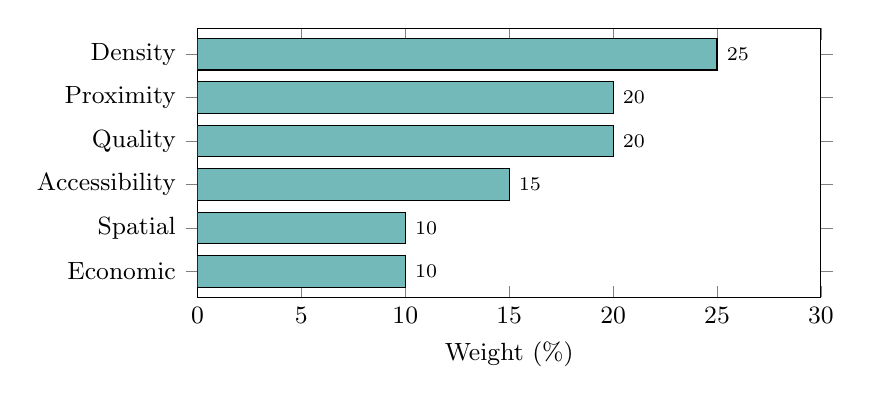
\begin{tikzpicture}
\begin{axis}[
  xbar, width=9.5cm, height=5cm, bar width=0.4cm,
  xlabel={Weight (\%)},
  symbolic y coords={Economic,Spatial,Accessibility,Quality,Proximity,Density},
  ytick=data, xmin=0, xmax=30,
  nodes near coords, nodes near coords align={horizontal},
  every node near coord/.style={font=\scriptsize},
  tick label style={font=\small}, label style={font=\small},
  enlarge y limits=0.12,
]
\addplot[fill=teal!55] coordinates {
  (10,Economic)(10,Spatial)(15,Accessibility)(20,Quality)(20,Proximity)(25,Density)
};
\end{axis}
\end{tikzpicture}
\caption{Six scoring components and their weights}
\end{figure}

\subsection{Component 1 --- Multi-Radius Weighted Density (25\%)}

\textbf{Multi-Radius Weighted Score:}
To capture both immediate walkability and regional availability, the density score is a weighted sum of scores at three radii:
\begin{align}
\text{Density Score} &= 0.5 \times S_{500\text{m}} + 0.3 \times S_{1\text{km}} + 0.2 \times S_{2\text{km}}
\end{align}
Each radius score $S_r$ is calculated against calibrated thresholds for that specific area size.
\begin{itemize}
    \item \textbf{500m (50\%):} Walkable / Immediate access.
    \item \textbf{1km (30\%):} Neighbourhood / Short drive.
    \item \textbf{2km (20\%):} Regional catchment.
\end{itemize}

\begin{table}[H]
\centering
\caption{Density thresholds calibrated to Indian urban data (95th percentile)}
\begin{tabular}{@{}lrr@{}}
\toprule
\textbf{Category} & \textbf{Threshold $\rho_0$} & \textbf{Score = 100 at $3\rho_0$} \\ \midrule
Essential   & 5.0 & 15.0 \\
Healthcare  & 2.5 & 7.5  \\
Education   & 1.5 & 4.5  \\
Transport   & 1.2 & 3.6  \\
Finance     & 2.0 & 6.0  \\
Shopping    & 5.0 & 15.0 \\
Food        & 3.5 & 10.5 \\
Cultural    & 2.5 & 7.5  \\
Premium     & 1.2 & 3.6  \\
Employment  & 0.5 & 1.5  \\
Civic       & 0.7 & 2.1  \\ \bottomrule
\end{tabular}
\end{table}

\subsection{Component 2 --- Proximity (20\%)}

\textbf{Formula (Exponential Decay):}
Proximity scoring focuses strictly on the \textbf{nearest} amenity, as this dictates immediate accessibility for urgent needs.
\begin{equation}
\text{Proximity Score} = 100 \times e^{-\lambda \cdot d_{\min}}
\end{equation}
Where $\lambda$ (decay rate) is calibrated per category (typically 1.5). This ensures a sharp drop-off: accessible within 1km scores well, while anything beyond 2km scores near zero.

\textbf{Basis --- Alonso's Bid-Rent Theory:} Value and utility drop exponentially with distance. The system prioritises the closest facility.

% Proximity decay curve
\begin{figure}[H]
\centering
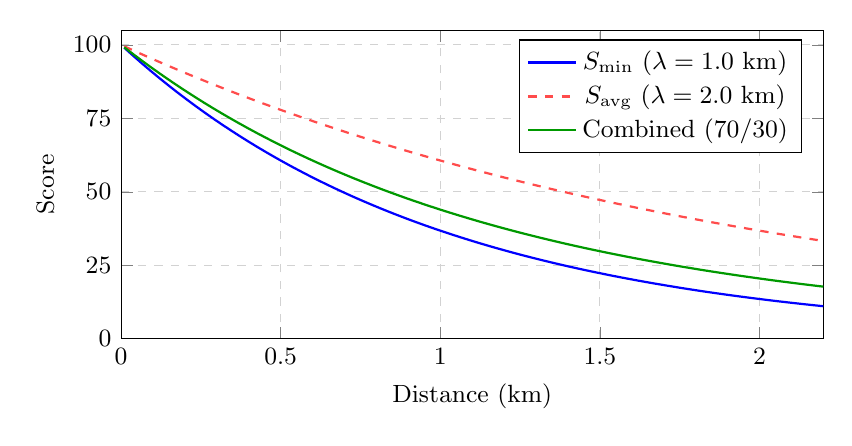
\begin{tikzpicture}
\begin{axis}[
  width=10.5cm, height=5.5cm,
  xlabel={Distance (km)}, ylabel={Score},
  xmin=0, xmax=2.2, ymin=0, ymax=105,
  xtick={0,0.5,1.0,1.5,2.0}, ytick={0,25,50,75,100},
  grid=major, grid style={dashed,gray!35},
  tick label style={font=\small}, label style={font=\small},
  legend pos=north east, legend style={font=\small},
]
\addplot[blue,  thick, domain=0.01:2.2, samples=80] {100*exp(-x/1.0)};
\addplot[red!70,thick, dashed, domain=0.01:2.2, samples=80] {100*exp(-x/2.0)};
\addplot[green!60!black, thick, domain=0.01:2.2, samples=80]
  {0.7*100*exp(-x/1.0)+0.3*100*exp(-x/2.0)};
\legend{$S_{\min}$ ($\lambda=1.0$ km), $S_{\text{avg}}$ ($\lambda=2.0$ km), Combined (70/30)}
\end{axis}
\end{tikzpicture}
\caption{Proximity score decay: combined score = 70\% nearest + 30\% average distance}
\end{figure}

\begin{table}[H]
\centering
\caption{Proximity score vs.\ distance}
\begin{tabular}{@{}lrrp{5.5cm}@{}}
\toprule
\textbf{Distance} & $S_{\min}$ & $S_{\text{avg}}$ & \textbf{Interpretation} \\ \midrule
0.1 km & 90.5 & 95.1 & Excellent --- 1 min walk \\
0.3 km & 74.1 & 86.1 & Very good --- 3 min walk \\
0.5 km & 60.7 & 77.9 & Good --- 5 min walk \\
1.0 km & 36.8 & 60.7 & Acceptable --- 12 min walk \\
1.5 km & 22.3 & 47.2 & Poor --- vehicle required \\
2.0 km & 13.5 & 36.8 & Very poor --- must drive \\ \bottomrule
\end{tabular}
\end{table}

\subsection{Component 3 --- Quality (20\%)}

\begin{equation}
r = \frac{N_{\text{premium}}}{N_{\text{basic}} + 1}
\end{equation}

\begin{equation}
\text{Quality Score} = \min\left(100, \left( \frac{N_{\text{premium}}}{N_{\text{total}}} \times 1.5 + \frac{N_{\text{basic}}}{N_{\text{total}}} \times 0.5 \right) \times 100 \right)
\end{equation}

Premium amenities (hospitals, universities, malls) are weighted 3x higher than basic ones (clinics, schools, stores). A location with only premium amenities scores 150 (capped at 100), ensuring that high-quality infrastructure is rewarded even if counts are lower.

\textbf{Healthcare example} ($r_L=0.3$, $r_M=0.8$, $r_H=1.5$):

\begin{center}
\begin{tabular}{@{}lll@{}}
\toprule
\textbf{Ratio} & \textbf{Score} & \textbf{Interpretation} \\ \midrule
$< 0.3$    & 20--50  & Basic --- clinics only \\
$0.3-0.8$  & 50--75  & Good --- some hospitals \\
$0.8-1.5$  & 75--90  & Excellent --- hospital hub \\
$> 1.5$    & 90--100 & Premium --- medical city \\ \bottomrule
\end{tabular}
\end{center}

\subsection{Component 4 --- Accessibility (15\%)}

\begin{align}
G &= \sum_{i=1}^{n} \frac{w_i}{\max(d_i, 0.1)^2} \\[6pt]
\text{Score} &= \min\left(100, G \right)
\end{align}

$w_i$ = importance weight; $d_i$ = distance in km (floor at 100m).
The raw gravity sum $G$ is normalised against a benchmark of 100 (e.g., dense urban baseline). This linear scaling provides a clearer gradient than the previous log-based approach.

$w_i$ = importance weight (premium POI = 3.0, standard = 1.0); $G_{\min}=0.1$ (rural baseline); $G_{\max}=100$ (city centre baseline).

\textbf{Basis --- Reilly's Law of Retail Gravitation (1931):} Interaction $\propto \text{mass}/\text{distance}^2$. Closer and higher-quality amenities contribute more to the score.

\textbf{Example:}

\begin{center}
\begin{tabular}{@{}llr@{}}
\toprule
\textbf{POI} & \textbf{Distance} & \textbf{Contribution ($w/d^2$)} \\ \midrule
Hospital ($w=3.0$) & 0.5 km & $3.0/0.25 = 12.0$ \\
Hospital ($w=3.0$) & 0.8 km & $3.0/0.64 = 4.7$  \\
Clinic   ($w=1.5$) & 0.3 km & $1.5/0.09 = 16.7$ \\
Pharmacy ($w=1.0$) & 0.2 km & $1.0/0.04 = 25.0$ \\ \midrule
\multicolumn{2}{@{}l}{Total gravity $G = 58.4$} &
  Score $= 100\times\dfrac{1.766+1}{3} = 92.2$ \\ \bottomrule
\end{tabular}
\end{center}

\subsection{Component 5 --- Spatial (10\%)}

\begin{equation}
\text{Spatial Score} = 0.70 \times S_{\text{Hotspot}} + 0.30 \times S_{\text{NNI}}
\end{equation}

\textbf{Rationale:}
\begin{itemize}
    \item \textbf{Hotspot Intensity (70\%):} Measures the size of the largest amenity cluster (DBSCAN). Large clusters indicate walkability.
    \item \textbf{NNI (30\%):} Global clustering metric. NNI $<1$ indicates non-random clustering.
\end{itemize}
We removed separate DBSCAN/Moran's I components to simplify the signal: if a strong hub exists (Hotspot) and amenities are clustered (NNI), the spatial layout is efficient.

\textbf{NNI sub-score:}
\begin{equation}
S_{\text{NNI}} = \begin{cases}
50 + \dfrac{\text{NNI}}{0.5}\times 50
  & \text{NNI} < 0.5 \\[6pt]
100
  & 0.5 \le \text{NNI} \le 1.0 \\[6pt]
100 - \dfrac{\text{NNI}-1.0}{0.5}\times 50
  & 1.0 < \text{NNI} \le 1.5 \\[6pt]
\max\!\bigl(0,\;50 - (\text{NNI}-1.5)\times 20\bigr)
  & \text{NNI} > 1.5
\end{cases}
\end{equation}

\textbf{Moran's I sub-score:}
\begin{equation}
S_{\text{Moran}} = \frac{I + 1}{2}\times 100
\quad\text{(maps $[-1,+1]$ to $[0,100]$)}
\end{equation}

\textbf{DBSCAN and Hotspot sub-scores:}
\begin{align}
S_{\text{DBSCAN}}  &= \frac{n_{\text{clusters}}}{n_{\text{POIs}}}\times 100 \\[4pt]
S_{\text{Hotspot}} &= \frac{\max(\text{cluster sizes})}{n_{\text{POIs}}}\times 100
\end{align}

\subsection{Component 6 --- Economic (10\%)}

\begin{equation}
p_{\text{actual}} = \frac{N_{\text{category}}}{N_{\text{total}}}\times 100
\end{equation}

\begin{equation}
\text{Ratio} = \frac{\text{Actual Share \%}}{\text{Target Share \%}}
\end{equation}

\begin{equation}
\text{Economic Score} = \frac{100}{1 + e^{-4(\text{Ratio} - 1.0)}}
\end{equation}

\textbf{Sigmoid Curve:} 
\begin{itemize}
    \item \textbf{Ratio = 1.0 (On Target):} Score = 50.
    \item \textbf{Ratio > 1.0 (Over-supply):} Rapidly approaches 100.
    \item \textbf{Ratio < 0.5 (Under-supply):} Drops towards 0.
\end{itemize}
This smooths the penalty for minor deviations while severely penalising missing sectors.

$p_a$ = actual share; $p_t$ = India-calibrated target share.

\begin{table}[H]
\centering
\caption{Target POI distribution (India-calibrated)}
\begin{tabular}{@{}lr@{}}
\toprule
\textbf{Category} & \textbf{Target \%} \\ \midrule
Essential   & 17 \\
Shopping    & 15 \\
Food        & 12 \\
Employment  & 12 \\
Transport   & 10 \\
Healthcare  & 8  \\
Cultural    & 8  \\
Education   & 6  \\
Finance     & 5  \\
Premium     & 4  \\
Civic       & 3  \\ \bottomrule
\end{tabular}
\end{table}

% ─────────────────────────────────────────────────────────────────────────────
\section{Penalty System}
% ─────────────────────────────────────────────────────────────────────────────

\subsection{Additive Framework}

After computing the base amenity index, four additive penalties are applied:

\begin{align}
\text{Total Penalty} &= \min\!\bigl(0.50,\;P_{\text{data}} + P_{\text{Gini}} + P_{\text{Simp}} + P_{\text{cat}}\bigr) \\[4pt]
\text{Final Score}   &= \text{Base Score}\times(1 - \text{Total Penalty})
\end{align}

Penalties are added together (not multiplied) and capped at 50\% to avoid over-penalising rural areas with limited data.

% Penalty stacking diagram
\begin{figure}[H]
\centering
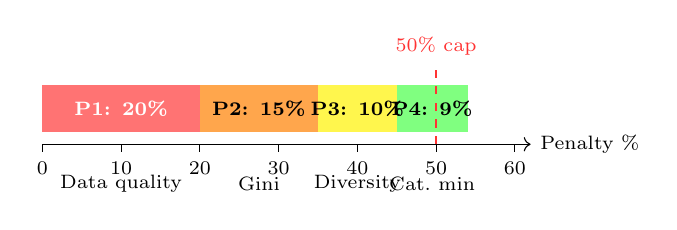
\begin{tikzpicture}[font=\small]
  % Draw stacked bar segments (each 1 unit = 10%)
  \fill[red!55]    (0,0) rectangle (2.0,0.6);   % P1: 20%
  \fill[orange!70] (2.0,0) rectangle (3.5,0.6); % P2: 15%
  \fill[yellow!70] (3.5,0) rectangle (4.5,0.6); % P3: 10%
  \fill[green!50]  (4.5,0) rectangle (5.4,0.6); % P4: 9%
  % Cap line at 50% = 5.0
  \draw[dashed, thick, red!80] (5.0,-0.15) -- (5.0,0.85)
    node[above, font=\scriptsize, red!80] {50\% cap};
  % Labels inside bars
  \node[white, font=\scriptsize\bfseries] at (1.0,0.3) {P1: 20\%};
  \node[font=\scriptsize\bfseries]        at (2.75,0.3){P2: 15\%};
  \node[font=\scriptsize\bfseries]        at (4.0,0.3) {P3: 10\%};
  \node[font=\scriptsize\bfseries]        at (4.95,0.3){P4: 9\%};
  % Axis
  \draw[->] (0,-0.15) -- (6.2,-0.15) node[right,font=\scriptsize] {Penalty \%};
  \foreach \x/\v in {0/0,1/10,2/20,3/30,4/40,5/50,6/60}
    \draw (\x,-0.15)--(\x,-0.25) node[below,font=\scriptsize]{\v};
  % Legend below
  \node[font=\scriptsize] at (1.0,-0.65)  {Data quality};
  \node[font=\scriptsize] at (2.75,-0.65) {Gini};
  \node[font=\scriptsize] at (4.0,-0.65)  {Diversity};
  \node[font=\scriptsize] at (4.95,-0.65) {Cat.\ min};
\end{tikzpicture}
\caption{Maximum penalty contributions (stacked), hard-capped at 50\%}
\end{figure}

\subsection{Penalty Definitions}

\textbf{P1 --- Data Quality (0--20\%):}
\begin{equation}
P_{\text{data}} = \begin{cases}
0.20 & n_{\text{POIs}} < 5 \\
0.10 & 5  \le n < 20 \\
0.05 & 20 \le n < 40 \\
0.00 & n \ge 40
\end{cases}
\end{equation}
Low counts may mean the area is under-mapped in OSM, not that amenities are truly absent.

\medskip
\textbf{P2 --- Gini Inequality (0--15\%):}
\begin{equation}
P_{\text{Gini}} = G \times 0.15, \quad G \in [0,1]
\end{equation}
When one category dominates, the area is unbalanced and less livable.

\medskip
\textbf{P3 --- Simpson Diversity (0--10\%):}
\begin{equation}
P_{\text{Simp}} = (1 - D)\times 0.10, \quad D \in [0,1]
\end{equation}
Low diversity means the area has mostly one type of amenity; mixed areas score higher.

\medskip
\textbf{P4 --- Category Minimum (0--9\%):}
\begin{equation}
P_{\text{cat}} = \min(0.09,\;0.03\times n_{\text{missing}})
\end{equation}
$n_{\text{missing}}$ = number of essential categories (Essential, Healthcare, Transport) with score $<10$. Each missing category adds a 3\% penalty.

% ─────────────────────────────────────────────────────────────────────────────
\section{Final Aggregation \& Classification}
% ─────────────────────────────────────────────────────────────────────────────

\begin{align}
\text{Base Index}  &= \sum_{c=1}^{11} w_c \times \text{Score}_c \\[4pt]
\text{Final Index} &= \text{Base Index}\times(1 - \text{Total Penalty})
\end{align}

\begin{equation}
\text{Classification} = \begin{cases}
\text{Metro} & \text{Index} \ge 60 \\
\text{Urban} & 30 \le \text{Index} < 60 \\
\text{Rural} & \text{Index} < 30
\end{cases}
\end{equation}

% Classification number line
\begin{figure}[H]
\centering
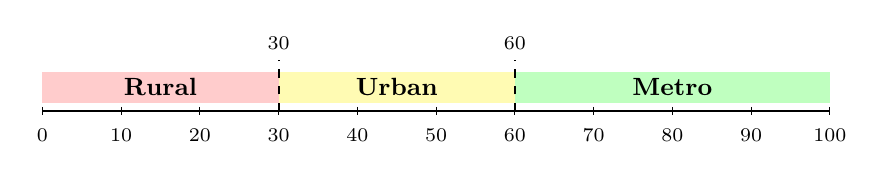
\begin{tikzpicture}[font=\small]
  \fill[red!20]    (0,0.1) rectangle (3,0.5);
  \fill[yellow!30] (3,0.1) rectangle (6,0.5);
  \fill[green!25]  (6,0.1) rectangle (10,0.5);
  \draw[thick] (0,0) -- (10,0);
  \foreach \x in {0,1,...,10}
    \draw (\x,0.05)--(\x,-0.05);
  \foreach \x/\v in {0/0,1/10,2/20,3/30,4/40,5/50,6/60,7/70,8/80,9/90,10/100}
    \node[below,font=\scriptsize] at (\x,-0.1) {\v};
  \node[font=\small] at (1.5,0.3) {\textbf{Rural}};
  \node[font=\small] at (4.5,0.3) {\textbf{Urban}};
  \node[font=\small] at (8.0,0.3) {\textbf{Metro}};
  \draw[dashed,thick] (3,0)--(3,0.65) node[above,font=\scriptsize]{30};
  \draw[dashed,thick] (6,0)--(6,0.65) node[above,font=\scriptsize]{60};
\end{tikzpicture}
\caption{Classification thresholds on the 0--100 amenity index scale}
\end{figure}

\begin{center}
\begin{tabular}{@{}ll@{}}
\toprule
\textbf{Class} & \textbf{Interpretation} \\ \midrule
Metro & Good coverage, easy access, mixed-use area \\
Urban & Moderate coverage, some gaps in services \\
Rural & Few amenities; travel needed for most services \\ \bottomrule
\end{tabular}
\end{center}

% ─────────────────────────────────────────────────────────────────────────────
\section{Validation Results (v1.0)}
% ─────────────────────────────────────────────────────────────────────────────

\begin{table}[H]
\centering
\caption{Dataset statistics (1,010 locations)}
\begin{tabular}{@{}lr@{}}
\toprule
\textbf{Metric} & \textbf{Value} \\ \midrule
Total locations        & 1,010 \\
Mean Amenity Index     & 48.2 \\
Median Amenity Index   & 49.0 \\
Std. Deviation         & 23.2 \\
Skewness               & -0.34 \\
Kurtosis              & -0.79 \\
Zero-Score Locations   & 34 (3.4\%) \\ \bottomrule
\end{tabular}
\end{table}

\subsection{Amenity Index Distribution}

\begin{figure}[H]
\centering
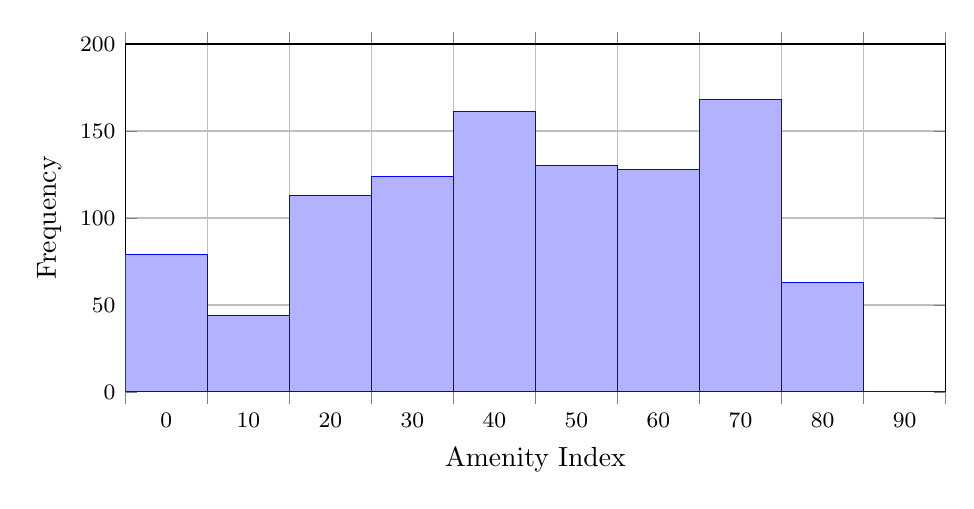
\begin{tikzpicture}
\begin{axis}[
    ybar interval,
    width=12cm, height=6cm,
    ymin=0, ymax=200,
    xmin=0, xmax=100,
    xlabel={Amenity Index},
    ylabel={Frequency},
    grid=major,
    xtick={0,10,20,30,40,50,60,70,80,90,100},
    tick label style={font=\footnotesize},
]
\addplot coordinates { 
    (0,79) (10,44) (20,113) (30,124) (40,161) 
    (50,130) (60,128) (70,168) (80,63) (90,0) (100,0) 
};
\end{axis}
\end{tikzpicture}
\caption{Distribution from 0-100 shows a balanced spread with a slight dip in the 80-90 range.}
\end{figure}

\subsection{Classification Analysis}

\begin{table}[H]
\centering
\caption{Descriptive Statistics by Classification}
\begin{tabular}{@{}lrrrrrrrr@{}}
\toprule
\textbf{Class} & \textbf{Count} & \textbf{\%} & \textbf{Mean} & \textbf{Median} & \textbf{Min} & \textbf{Max} & \textbf{Skew} & \textbf{Kurt} \\ \midrule
Metro & 359 & 35.5\% & 73.0 & 73.9 & 60.0 & 84.9 & -0.22 & -1.12 \\
Urban & 415 & 41.1\% & 44.8 & 46.5 & 30.0 & 60.0 & 0.01 & -1.12 \\
Rural & 235 & 23.3\% & 15.9 & 19.6 & 0.0 & 30.0 & -0.38 & -1.42 \\ \bottomrule
\end{tabular}
\end{table}

\subsection{Category Performance}

\begin{table}[H]
\centering
\caption{Detailed Category Statistics (Mean, Median, Dist.)}
\begin{tabular}{@{}lrrrrrr@{}}
\toprule
\textbf{Category} & \textbf{Mean} & \textbf{Median} & \textbf{P25} & \textbf{P75} & \textbf{Skew} & \textbf{Kurt} \\ \midrule
Essential   & 65.3 & 70.2 & 46.7 & 85.2 & -0.87 & 0.10 \\
Healthcare  & 62.1 & 65.3 & 42.1 & 85.0 & -0.66 & -0.72 \\
Education   & 48.4 & 49.6 & 20.3 & 76.3 & -0.24 & -1.12 \\
Transport   & 44.1 & 42.5 & 27.3 & 66.9 & -0.09 & -0.97 \\
Shopping    & 41.2 & 37.8 & 17.4 & 69.5 & 0.08 & -1.26 \\
Finance     & 36.0 & 34.5 & 0.0 & 61.6 & 0.22 & -1.27 \\
Employment  & 35.4 & 32.9 & 14.6 & 59.4 & 0.24 & -1.21 \\
Food        & 32.7 & 30.0 & 0.0 & 53.3 & 0.36 & -1.05 \\
Premium     & 37.5 & 36.5 & 0.0 & 58.2 & 0.23 & -1.04 \\
Civic       & 37.6 & 39.5 & 0.0 & 60.4 & 0.07 & -1.18 \\ \bottomrule
\end{tabular}
\end{table}

% ─────────────────────────────────────────────────────────────────────────────
\section{Limitations}

\subsection{Data Limitations}

\begin{enumerate}
  \item \textbf{OSM completeness.} Areas with less OSM data --- often rural --- may score lower than their actual amenity level.

  \item \textbf{Static data.} The system does not account for time-of-day changes, seasonal businesses, opening hours, or recent openings and closures.

  \item \textbf{No quality data.} All POIs of the same type are treated equally --- no distinction for hospital size, school ranking, or user ratings.
\end{enumerate}

\subsection{Methodological Limitations}

\begin{enumerate}
  \item \textbf{Straight-line distance.} Haversine distances do not follow roads. Actual travel distances are typically 1.3--1.5$\times$ longer in urban areas; physical barriers like rivers or highways can increase this further.

  \item \textbf{India calibration.} Thresholds and weights are based on Indian urban data. Use in other countries requires recalibration.

  \item \textbf{Fixed 2 km radius.} The radius may be too small for rural areas and too large for dense city centres. It does not adjust based on local transport.

  \item \textbf{Weight assumptions.} Category weights are based on Maslow's hierarchy and may not fit all regions (e.g., tourism or employment-heavy areas).
\end{enumerate}

\subsection{Technical Limitations}

\begin{enumerate}
  \item \textbf{API dependency.} The system needs the OSM Overpass API. While v1.0 includes robust retries, extreme network issues or API downtime can still block fresh data fetching.

  \item \textbf{Cache staleness.} The 30-day cache improves speed but may miss recent POI changes until the cache refreshes.

  \item \textbf{Processing speed.} Batch processing 1,010 locations takes approx 20--30 minutes due to polite API throttling (2 req/s) and retry overrides for difficult locations.

  \item \textbf{Unused features.} Over 1,000 features are extracted (temporal, brand presence, detailed curves), but only $\approx$280 are currently used in the scoring model. The rest are reserved for future ML enhancements.
\end{enumerate}

\end{document}
